
\documentclass{article}

% If you're new to LaTeX, here's some short tutorials:
% https://www.overleaf.com/learn/latex/Learn_LaTeX_in_30_minutes
% https://en.wikibooks.org/wiki/LaTeX/Basics

% Formatting
\usepackage[utf8]{inputenc}
\usepackage[margin=1in]{geometry}
\usepackage[titletoc,title]{appendix}

% Math
% https://www.overleaf.com/learn/latex/Mathematical_expressions
% https://en.wikibooks.org/wiki/LaTeX/Mathematics
\usepackage{amsmath,amsfonts,amssymb,mathtools}

% Images
% https://www.overleaf.com/learn/latex/Inserting_Images
% https://en.wikibooks.org/wiki/LaTeX/Floats,_Figures_and_Captions
\usepackage{graphicx,float}

% Tables
% https://www.overleaf.com/learn/latex/Tables
% https://en.wikibooks.org/wiki/LaTeX/Tables

% Algorithms
% https://www.overleaf.com/learn/latex/algorithms
% https://en.wikibooks.org/wiki/LaTeX/Algorithms
\usepackage[ruled,vlined]{algorithm2e}
\usepackage{algorithmic}

% Code syntax highlighting
% https://www.overleaf.com/learn/latex/Code_Highlighting_with_minted
\usepackage{minted}
\usemintedstyle{borland}

% References
% https://www.overleaf.com/learn/latex/Bibliography_management_in_LaTeX
% https://en.wikibooks.org/wiki/LaTeX/Bibliography_Management
\usepackage{biblatex}
\addbibresource{references.bib}
\usepackage[euler]{textgreek}
\usepackage{url}
\usepackage{hyperref}
\usepackage{float}
\usepackage{siunitx}
\renewcommand \thesubsubsection {\Alph{subsubsection}}
\renewcommand{\thesubsubsection}{\alph{subsubsection})}
\makeatletter
\renewcommand{\p@subsubsection}{\thesubsection.\protect\eatbracket}


% Title content
\title{EE 462 Homework 1}
\author{Burak Kemal Kara}
\date{March 21, 2020}

\begin{document}
\begin{titlepage}
    \begin{center}
        \vspace*{1cm}
            
        \Huge
        \textbf{DC/DC Voltage Regulator}
            
        \vspace{0.5cm}
        \LARGE
        Complete Simulation Report
            
        \vspace{1.5cm}
            
        \textbf{Cemil Ürgüp}\\
        \textbf{Burak Kemal Kara}
            
        \vfill
            
        A report presented for the sake of\\
        Humanity and Science
            
        \vspace{0.8cm}
            
        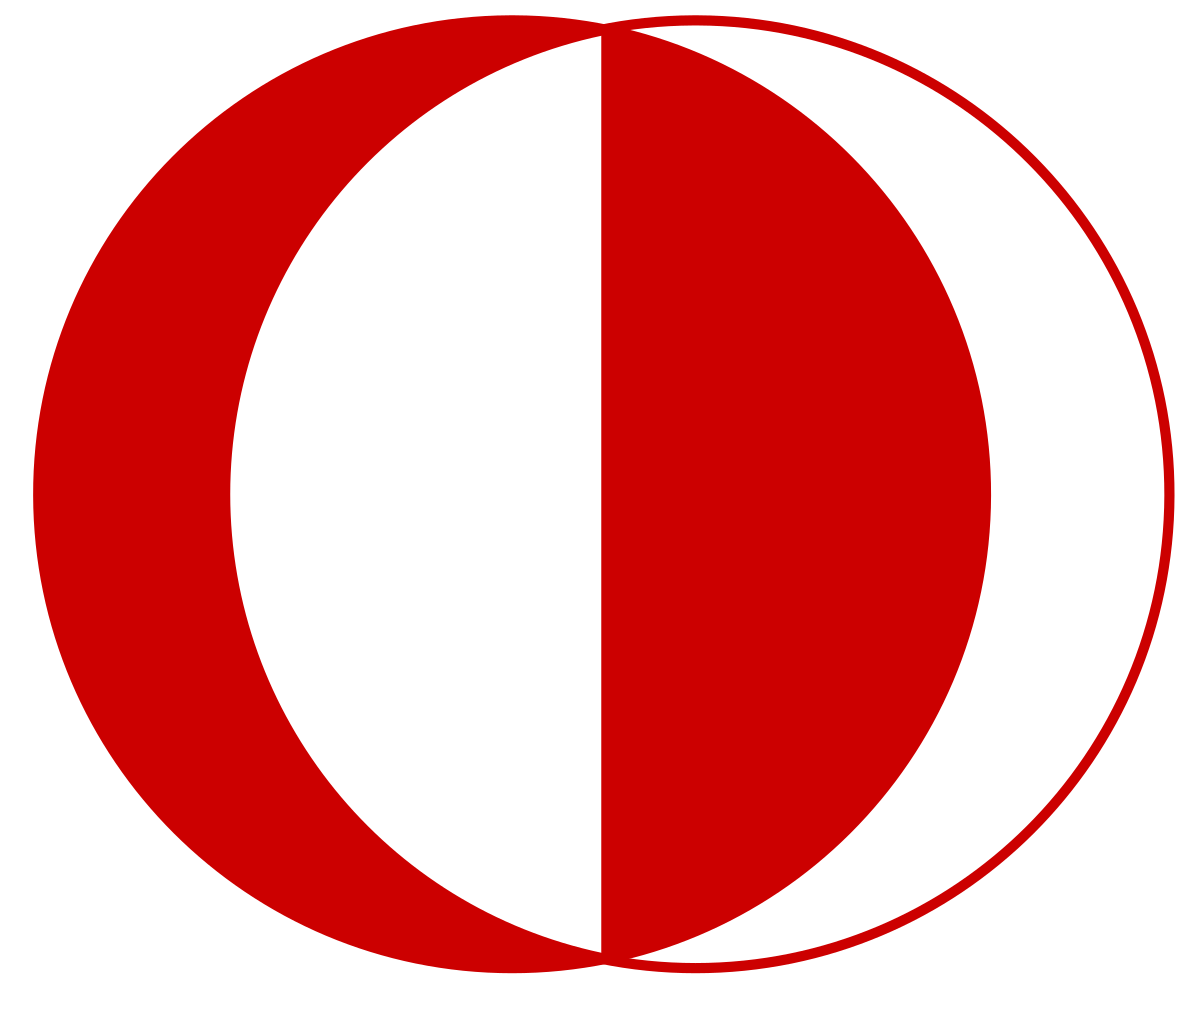
\includegraphics[width=0.4\textwidth]{logo.png}
            
        \Large
        Electrical \& Electronics Engineering\\
        MIDDLE EAST TECHNICAL UNIVERSITY\\
        TURKEY\\
        23.03.2020
            
    \end{center}
\end{titlepage}
%Table of contents
\tableofcontents
\newpage
%Introduction
\section{Introduction}
Switch mode power supplies are commonly used to DC/DC converter applications. 
Beside of voltage control, it provides galvanic isolations. 
In this project we used Forward Converter topology which is good choice when output need high current and power range is below 200W. 
This document aims to discuss component selections according to teoric and computational simulation results.
\section{Forward Converter topology}
\section{Design Equations}
The following specifications are design equtions for Forward Converter Design.
\begin{table}[H]
    \centering
\begin{tabular}{|l|l|}
    \hline
    Minimum Input Voltage (V)             & 24      \\ \hline
    Maximum Input Voltage (V)             & 48      \\ \hline
    Output Voltage (V)                    & 15      \\ \hline
    Output Power (W)                      & 48      \\ \hline
    Output Volt. Peak-to-Peak Ripple (\%) & 2       \\ \hline
    Switching Frequency (fs)              & 100 kHz \\ \hline
\end{tabular}
\end{table}
%Transformer
\subsection{Transformer Considerations}
First of all we should calculate turn ratio of transformer. For the sake of simplicity reset winding and primary winding ratio is same.
\begin{equation}
    n_{1}=n_{3}
\end{equation}
This equation limit max duty ratio to 50\%, since core cant demagnetize faster than magnetizing time.
Primary and secondary winding ratio can found when critical points are considered. When Input decreased minumum, Duty cycle reached max. ratio.At this point this converter should supply desired $V_o$.
\begin{equation}
    V_o<v_i\frac{n_3}{n_1}D \quad \implies \quad \frac{n_3}{n_1}>\frac{V_o}{V_i\cdot D}=1.33 \implies 2
\end{equation}
When $V_o=15 V$ as specifications, extra voltage drop on $D_2$ around 1V. \\$V_{o,max}=16 V$.\\Minimum voltage is 24 V. \\Maximum D is 50\%.\\
At this point we choose R type material ferrite core (Code:0R45959EC). We selected since,R type core loss is less than P type core. According to this core turning factor can found from Lenz Rule,
\begin{equation}
    V=n_1\frac{d\phi}{dt} \implies V_{i,max}=\frac{n_1\cdot B_{sat}\cdot A_e}{D{max}\cdot T_s}
\end{equation}
\[\therefore n_1> 2.18\]
$V_{i,max}$=48 V\\
$D_{max}$=0.5\\
$B_{sat}$=0.3\\
$A_e= 368 mm^2$ taken from datasheet \cite{core}.\\
This is minimum turning ratio to avoid core saturation.
To calculate max turn number we should calculate wire type to know wire size.
At the worst scenario we have $V_{in,min}=24 V$. For primary winding,
\begin{equation}
    I_{primary}=\frac{P_o}{V_{in,min}}=2A
\end{equation}
For secondary winding,
\begin{equation}
    I_{secondary}=\frac{I_{primary}}{n}=1A
\end{equation}
Since this currents ratings are for ideal case, it is safer to choose higher rating wires.From AWG chart,for primary and reset windings can use AWG \#16, Secondary AWG \#18. Selection criteria is max current. Their properties are shown at table 2.
\begin{table}[H]
    \centering
\begin{tabular}{|l|l|l|}
    \hline
    \multicolumn{1}{|c|}{AWG} & \multicolumn{1}{c|}{\begin{tabular}[c]{@{}c@{}}Area\\ mm\textasciicircum{}2\end{tabular}} & \multicolumn{1}{c|}{\begin{tabular}[c]{@{}c@{}}Max. Current \\ Amperes\end{tabular}} \\ \hline
    AWG\#16                   & 1.31                                                                                      & 3.7                                                                                  \\ \hline
    AWG\#18                   & 0.823                                                                                     & 2.3                                                                                  \\ \hline
    \end{tabular}
\end{table}
Core window area is calculated from datasheet.Also geometry parameters are taken from datasheet \cite{core}.
\begin{equation}
    A_{w}=(E-F)\cdot D=510 mm^2
\end{equation}
Since area of wires are known max turn can be calculate by,
\begin{equation}
    N_{max}=\frac{k_{fill}\cdot A_w}{A_{pri}+n\cdot A_{sec}+A_{reset}}=71.73
\end{equation}
Note that fill factor is 0.3 for litz wire.Increasıng turn is good because flux density decreasing and core loss decreasing according to Steinmetz equation, but increased turn also increase resistance of wire and copper loss increased.
Core loss equation,
\begin{equation}
    P_{fe}=K_{fe}(B_{peak})^\beta A_cl_m
\end{equation}
$P_{fe}$ at 100kHz,100mT given $85mW/cm^3$\\
$P_{fe}$ at 100kHz,200mT given $550mW/cm^3$\\By using these values steinmetz parameters calculated as,\\
\[\therefore \beta =2.7 \quad ,K_{fe}=42\]
Core loss is simply $I^2R_{ac}$ but wires new resistance should be calcualted by skin effect.Since skin depth decrease wire area new resistance calculated by,
\begin{equation}
    R_{ac}=\frac{n\cdot MLT \cdot \rho}{Area }
\end{equation}
To find optimum turn number loss calculated at matlab script which provided at github repo.
\begin{figure}[H]
    \centering
    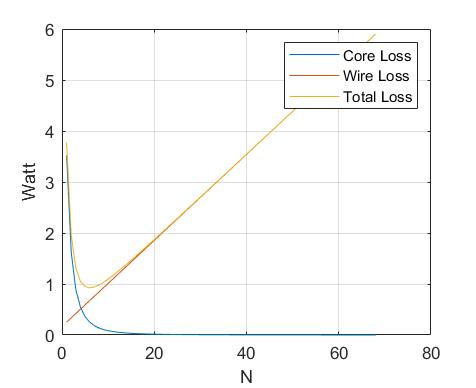
\includegraphics[width=0.5\linewidth]{number.jpg}
    \caption {According to number of turn Total loss calculated}
    \label{fig:sepic_cap_ideal}
\end{figure}
It is better to select turn ratio 8 which Total loss is 1 Watt.
At this number $R_{pri}=R_{reset}=0.05 k\Omega$, $R_{sec}=0.06 k\Omega$.\\
By using AL number windings inductance found and,
\begin{equation}
    X_m=k\cdot \sqrt{X_1\cdot (X_2+X_3)}=637 \mu H 
\end{equation}
Since reset and secondary windings direction same they summed. Also from Steinmetz eqn. $R_m$ can found.Where applied voltage is 48 V.
\begin{equation}
    P_{fe}=0.1375 Watt \implies R_m=\frac{V^2}{P_{fe}}=16.7k\Omega
\end{equation}
\subsection{MOSFET Considerations}
Since when switch is off, reset windig decharge core, beside of input voltage additional voltage seen on mosfet.
\begin{equation}
    V_s=V_i+\frac{n_1}{n_2}\cdot V_i=96 V
\end{equation}
For the worst case, selected $V_i=48V$. To be stay at the safe side lets make it 150V.
We aims to work in \%90 efficiency.Since $P_o=48 W$, $P_i=54 W$.At the minimum voltage max current created.
\begin{equation}
    I_i=\frac{P_i}{V_i}=2.22 A
\end{equation}
To be safe side minimum current of mosfet should be 5 A.
We selected to use IRF 740 N \cite{mosfet}, its voltage is 400V but since it has low resistance and it presents at available component list at the laboratory it is advantageous.
\\According to datasheet turn on and turn off time is 45ns.This much smaller than switching $t_off$ and $t_off$.
\begin{equation}
    P_{cond}=I_{i}^2\cdot R_{on}=2.7 W
\end{equation}
\begin{equation}
    P_{switching}=\frac{1}{2}\cdot V_{in}I_{in}(t_r+t_f)f_s=0.12W
\end{equation}
Conduction power loss is higher than expect, We can change this mosfet with better one at future. We will use this mosfet since we already have this component at the laboratory.
\subsection{Output Inductor Considerations}
\subsection{Capacitor Considerations}
\subsection{Diode Considerations}
\section{References}
\printbibliography
\end{document}
